\documentclass{llncs}

\usepackage{graphicx}
\usepackage{url}
\usepackage{amsfonts}
\usepackage{moreverb}
%\usepackage[bookmarksnumbered=true,bookmarksopen=true,colorlinks,citecolor=red,pagebackref,hypertexnames=true]{hyperref}
\usepackage[bookmarksnumbered=true,colorlinks,citecolor=blue,urlcolor=blue]{hyperref}

% so we don't need to specify figures subdirectory in figure code
\graphicspath{{./figures/}}
\usepackage{subfig}

%needed to change table colors
\usepackage[table]{xcolor}

%\usepackage{wrapfig}
\usepackage{bm}
\usepackage{paralist}
\usepackage{minted}

%
% Macro for comments
%
\def\mpar#1{\marginpar{\raggedright\scriptsize\sf #1}}
\renewcommand\verbatimtabsize{2\relax}

\newcommand{\anonymize}[2]{#1}


\begin{document}
\begin{sloppy}
\title{An Activity Monitoring System for Able-Bodied Humans and NAO Humanoid Robots using CSC688
Energia}
\author{Saminda Abeyruwan and Faisal Sikder}
\institute{University of Miami, Department of Computer Science,\\
1365 Memorial Drive, Coral Gables, FL, 33146, USA\\
E-Mail: {\ttfamily \{saminda|f.sikder\}@cs.miami.edu}
}

\maketitle

\begin{abstract}
CSC688 Energia is a software development platform for MSP-EXP430G2 LaunchPad, Tiva C Series
EK-TM4C123GXL LaunchPad, and Tiva C Series TM4C129 Connected LaunchPad. Our framework is
lightweight, flexible, and consumes minimum memory and computational resources to build
applications and rational agents on microcontrollers that sense and actuate using add-on boards. We
have used the framework to monitor activities such as standing, walking, and falling on able-bodied
humans and on NAO humanoid robots using thresholding and machine learning methods. We empirically
evaluate the outcomes and show the success of the methods on different activity scenarios.  
\end{abstract}


\section{Introduction}

Texas Instruments (TIs) microcontrollers and add-on boards such as MSP430{\texttrademark}
LaunchPad\footnote{\url{http://www.ti.com/tool/msp-exp430g2}},
Tiva{\texttrademark} C Series TM4C123G
LaunchPad\footnote{\url{http://www.ti.com/tool/ek-tm4c123gxl}} (a low-cost evaluation platform for
ARM
Cortex-M4F-based microcontrollers), Tiva C Series TM4C129 Connected
LaunchPad\footnote{\url{https://tinyurl.com/tm4c129}} (a new
development platform from Texas Instruments
based on the powerful TM4C129), and Sensor
Hub BoosterPack\footnote{\url{http://www.ti.com/tool/boostxl-senshub}} (an add-on board designed to
fit Tiva C Series TM4C123G LaunchPad
along with all of TI’s MCU LaunchPads) provide ultimate solutions
for a wide rage of low power and portable applications.

Therefore, a modular and flexible software
framework allow practitioners to use the functionalities provides by these systems effectively
and efficiently. This paper describes a software contribution that allows the development of
applications using open source principles and machine learning within
Energia\footnote{\url{http://energia.nu/}} open-source electronics prototyping platform.

The framework provides functionalities to build  rational agents that perceive its
environment though sensors and act upon it though actuators \cite{russel2009}. The execution path
between sensors to actuators may contain complex behaviors and modeling decisions that needs to be
handled carefully. Hence, the framework takes these consideration into account and provides a
topologically sorted graph based on the decision points provided by practitioners. Our
framework consists for four parts. It consists of modules and representations that execute on
\begin{inparaenum}[(1)]\item microcontrollers (incremental); \item offline (batch mode); \item NAO
robots\footnote{\url{http://www.aldebaran.com/en}}; and \item real-time
visualizations\end{inparaenum}. Our framework is lightweight, flexible, and consumes minimum memory
and computational resources as
possible. The framework also integrates RLLib, a C\texttt{++} template library that predict,
control, learn behaviors, and represent learnable knowledge using on/off policy reinforcement
learning, and supervised learning. Our framework, ``CSC688 Energia'', is publicly available from
GitHub repository \url{https://github.com/samindaa/csc688}.

We have tested our framework on multiple microcontrollers and on a sensor hub as stated above. We
have written and distributed software solutions to access devices on the sensor hub such as
\begin{inparaenum}[(1)] \item InvenSense MPU-9150: 9-axis MEMS motion tracking (3-axis gyro
3-axis accelerometer, and 3-axis compass); \item Bosch Sensortec BMP180 pressure sensor; \item
Sensirion SHT21 humidity and ambient temperature sensor; \item Intersil ISL29023 ambient and
infrared light sensor; and \item TIs TMP006 non-contact infrared temperature sensor\end{inparaenum}.

On the practical point-of-view, we have used our framework to experiment on the problem of activity
detection using InvenSense MPU-9150: 9-axis MEMS motion tracking sensor. We have conducted our
experiments on able-bodied humans and on NAO humanoid robots to detect motions such as standing,
walking, and abruptly falling back and front. We have used threshold based methods and machine
learning methods to detect these events and provide justifications, validations, and conclusions of
each method.  


\section{Software Architecture}

The software development framework uses a notion of ``modules'' and ``representations'' to perform
computations. The modules implement functions, while the representations exchange information from
one module to another. Figure \ref{fig:framework} shows an example of modules and representations
currently available in CSC688 Energia.

\begin{figure}[ht]
\centering
 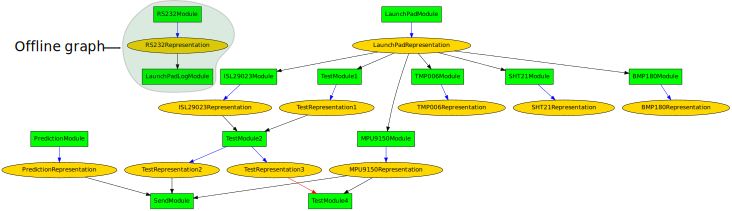
\includegraphics[width=1.0\textwidth] {framework}
 \caption{An example of modules and representations available in CSC688 Energia.}
 \label{fig:framework}
\end{figure}

The green boxes represent modules, while the yellow ellipses represent the representations. As an
example, the module {\sf MPU9150Module} contains logic to read/write from MPU-9150 Nine-Axis
(Gyro+Accelerometer+Compass) MEMS MotionTracking
device\footnote{\url{http://www.invensense.com/mems/gyro/mpu9150.html}} on the sensor hub booster
pack. The representation {\sf MPU9150Representation} contains all the values that the module
{\sf MPU9150Module} would like to share with other modules. In this graph, {\sf TestModule4}
requests
values from {\sf MPU9150Representation} to implement its logic. A module can provide multiple
representations as shown in the module {\sf TestModule2}. The blue arrows shows the provided
representations, the black arrows show the requested representations, and the red arrows show the
used representations.

There are two graphs in the figure; \begin{inparaenum}[(1)] \item the ``offline graph'' will be
executed offline, \item while the rest
of the graph, ``online graph'', will be executed on the devices\end{inparaenum}. We have shown only
two graphs in
this figure; in reality, one can keep up to $N$ number of graphs. The end uses of the software only
requires to write modules and representations, while the framework will compute the
topologically sorted graph out of the nodes. This will be computed once online/offline, and the
nodes in the queue will be executed one after the other. If there were to be cycles in the graph,
the framework will detect them and indicate them to the users.

The module {\sf PredictionModule} uses {\sf
RLLib}\footnote{\url{https://github.com/samindaa/RLLib}} library to learn, predict, and control
online on supervised and reinforcement learning problems. It provides
the representation {\sf PredictionRepresentation}. There exists a module {\sf SendModule} to send
values of the representations to offline modules. This is useful during the development phases of
a project. The module {\sf RS232Module} reads the data values that is send from {\sf SendModule}.
Please refere  to appendix for more information on implementations and
examples of the framework.

\section{Experiments \& Results}

We have conducted experiments on detecting motions (activities) on able-bodied humans and on NAO
humanoid robots. In order to detect motions, we have used InvenSense MPU-9150: 9-axis MEMS
motion tracking sensor on the sensor hub. The module {\sf MPU9150Module} connects to this device
and provides the representation {\sf MPU9150Representation}. The representation contains
3-axis accelerometer readings, 3-axis gyroscope readings, 3-axis magnetometer readings, quaternion
rotation axis of the device, and Euler angles roll, pitch, and yaw.  In order to calculate Euler
angles, we have used the Direction Cosine Matrix (DCM)
algorithm\footnote{\url{http://www.ti.com/lit/an/slaa518a/slaa518a.pdf}}.  Depending on the
experiment, the practitioner can change the sampling rate of the sensor.  The maximum sampling rate
of the sensor is 1000$Hz$. This section shows our results, validations, and conclusions.

\subsection{Able-Bodied Human}

We have collected data for different human activities. We have put the sensors on the chest of the
human body and collected data from those sensors in fixed interval. For this experiment, we have
sampled data in 50$Hz$ (or 20$ms$). We have data from several different human configurations:
\begin{inparaenum}[(1)] \item standing; \item seating; \item walking; \item standing to seating;
and \item standing to falling\end{inparaenum}. We have collected data based on the activities and
each data point has twelve fields, where nine fields are from nine reading from sensors and three
fields (yaw, pitch and roll) are derived from all those sensors reading.

\subsection*{Classification using Logistic Regression}

In the first part of the data analysis we have put all our collected data together and labeled it
with specific number to denote the position. We have used multivariate logistic regression model to
classify our data. We have used 80\% of the data for training, while the rest has been used
in validation.

\begin{table}[!h]
	\caption{Standing to seating detection.}	
	\label{tab:StandingToSeatingDetection}
	\centering
		\begin{tabular} {l l |c |c}
			& & Predict& Predict \\ 
			& & Seating & Standing \\ \hline
			Actual& Seating & 94 & 6\\ \hline
			Actual& Standing & 19& 81\\ \hline
		\end{tabular}
\end{table}

Table \ref{tab:StandingToSeatingDetection} shows the predictions of standing to seating position
movement for 200 data points. we can observe that we are able
to predict this movement with quite good accuracy (approximately 87.5\%). Table
 \ref{tab:StandingToWalkingDetection} shows the results for  standing to walking movement. In this
movement, our prediction accuracy is about 86\%. In the actual fall prediction logistic
regression can predict fall with 87.5\% accuracy (Shown in Table
 \ref{tab:StandingToFallingDetection}).
\vspace{-5mm}
\begin{table}
\caption{Standing to walking detection.}
	\label{tab:StandingToWalkingDetection}
\centering
		\begin{tabular} {l l |c |c}
			& & Predict& Predict \\ 
			& & Walking & Standing \\ \hline
			Actual& Walking & 89 & 11\\ \hline
			Actual& Standing & 17& 83\\ \hline
		\end{tabular}
\end{table}
\vspace{-10mm}
\begin{table}[!h]
\caption{Standing to falling detection.}
\label{tab:StandingToFallingDetection}
\centering
		\begin{tabular} {l l |c |c}
			& & Predict& Predict \\ 
			& & Fall & Standing \\ \hline
			Actual& Fall & 92 & 08\\ \hline
			Actual& Standing & 17& 83\\ \hline
		\end{tabular}
\end{table}
\vspace{-5mm}
\subsection*{Classification and Validation using Support Vector Machine}

In the second part of the data analysis, we have used support vector machine (SVM) model
to classify our data. To train the model, we used the same procedure as before, 80\% of
our data were used to do the classification and rest twenty percent data were used to validate our
classification result.

Table \ref{tab:StandingToSeatingDetectionsvm} shows the prediction of standing to seating position
movement for 200 data points. From that table we can observe that we are able to predict this
movement with quite good accuracy (approximately 90\%). Table
\ref{tab:StandingToWalkingDetectionsvm} shows the predictions for standing to
walking movement. In that movement our prediction accuracy is about 89.5\%. In the actual fall
prediction, SVM can predict fall with 90.5\% accuracy (Shown in Table
\ref{tab:StandingToFallingDetectionsvm}).
\vspace{-5mm}
\begin{table}[!h]
\caption{Standing to seating detection with SVM.}
	\label{tab:StandingToSeatingDetectionsvm}
	\centering
		\begin{tabular} {l l |c |c}
			& & Predict& Predict \\ 
			& & Seating & Standing \\ \hline
			Actual& Seating & 96 & 4\\ \hline
			Actual& Standing & 16& 84\\ \hline
		\end{tabular}
\end{table}
\vspace{-10mm}
\begin{table}[!h]
	\caption{Standing to walking detection with SVM.}
	\label{tab:StandingToWalkingDetectionsvm}
	\centering
		\begin{tabular} {l l |c |c}
			& & Predict& Predict \\ 
			& & Walking & Standing \\ \hline
			Actual& Walking & 93 & 07\\ \hline
			Actual& Standing & 14& 86\\ \hline
		\end{tabular}
\end{table}
\vspace{-10mm}
\begin{table}[!h]
	\caption{Standing to falling detection with SVM.}
	\label{tab:StandingToFallingDetectionsvm}
	\centering
		\begin{tabular} {l l |c |c}
			& & Predict& Predict \\ 
			& & Fall & Standing \\ \hline
			Actual& Fall & 95 & 05\\ \hline
			Actual& Standing & 14& 86\\ \hline
		\end{tabular}
\end{table}
\vspace{-5mm}
\subsection*{Fall Prediction within Time Frame}

A falling event does not happen within a single reading from sensors, it is consists of multiple
reading from sensors.  Its not really accurate to detect a fall or any other motion based on a
single reading, which might mislead the whole detection procedure. To detect a motion accurately we
have used a time frame based prediction procedure. In this procedure, we first train our SVM with
training data. Then we try to detection motion in each sensor reading. We will predict a motion not
based on a single reading but with all the reading within 100$ms$ time frame. If our detection
procedure detect a true fall event more than 90\% time, we will denote that event as a true
falling event. By applying the above algorithm, our predictions are 100\% accuracy.
Table \ref{tab:StandingToFallingDetectionsvmframe} shows detection of fall within 100$ms$ time
frame.

\begin{table}[!h]
\caption{Standing to falling detection within time frame.}
	\label{tab:StandingToFallingDetectionsvmframe}
	\centering
		\begin{tabular} {l l |c |c}
			& & Predict& Predict \\ 
			& & Fall & Standing \\ \hline
			Actual& Fall & 100 & 0\\ \hline
			Actual& Standing & 0& 100\\ \hline
		\end{tabular}
\end{table}

\subsection{NAO Humanoid Robot}

We have used Tiva C microcontroller with sensor hub attached to it to conduction our experiments in
this section. The device was first uploaded with CSC688 Energia to send information from device to
NAO though the serial port. The calculations were conducted on the device, while the outcomes were
serialized to the file system of NAO. We have integrated NAO software and CSC688 Energia to send and
received data from the device and the robot. Figure \ref{fig:attached_device}(a) shows the location
in which the device was attached. Figure \ref{fig:attached_device}(b) shows the Sensor Hub
BoosterPack. The roll is around x-axis, the pitch is around y-axis, and the yaw is around z-axis. 
We have used the USB port of the robot to communicate with the device.  


\begin{figure}[!ht]
\centering
 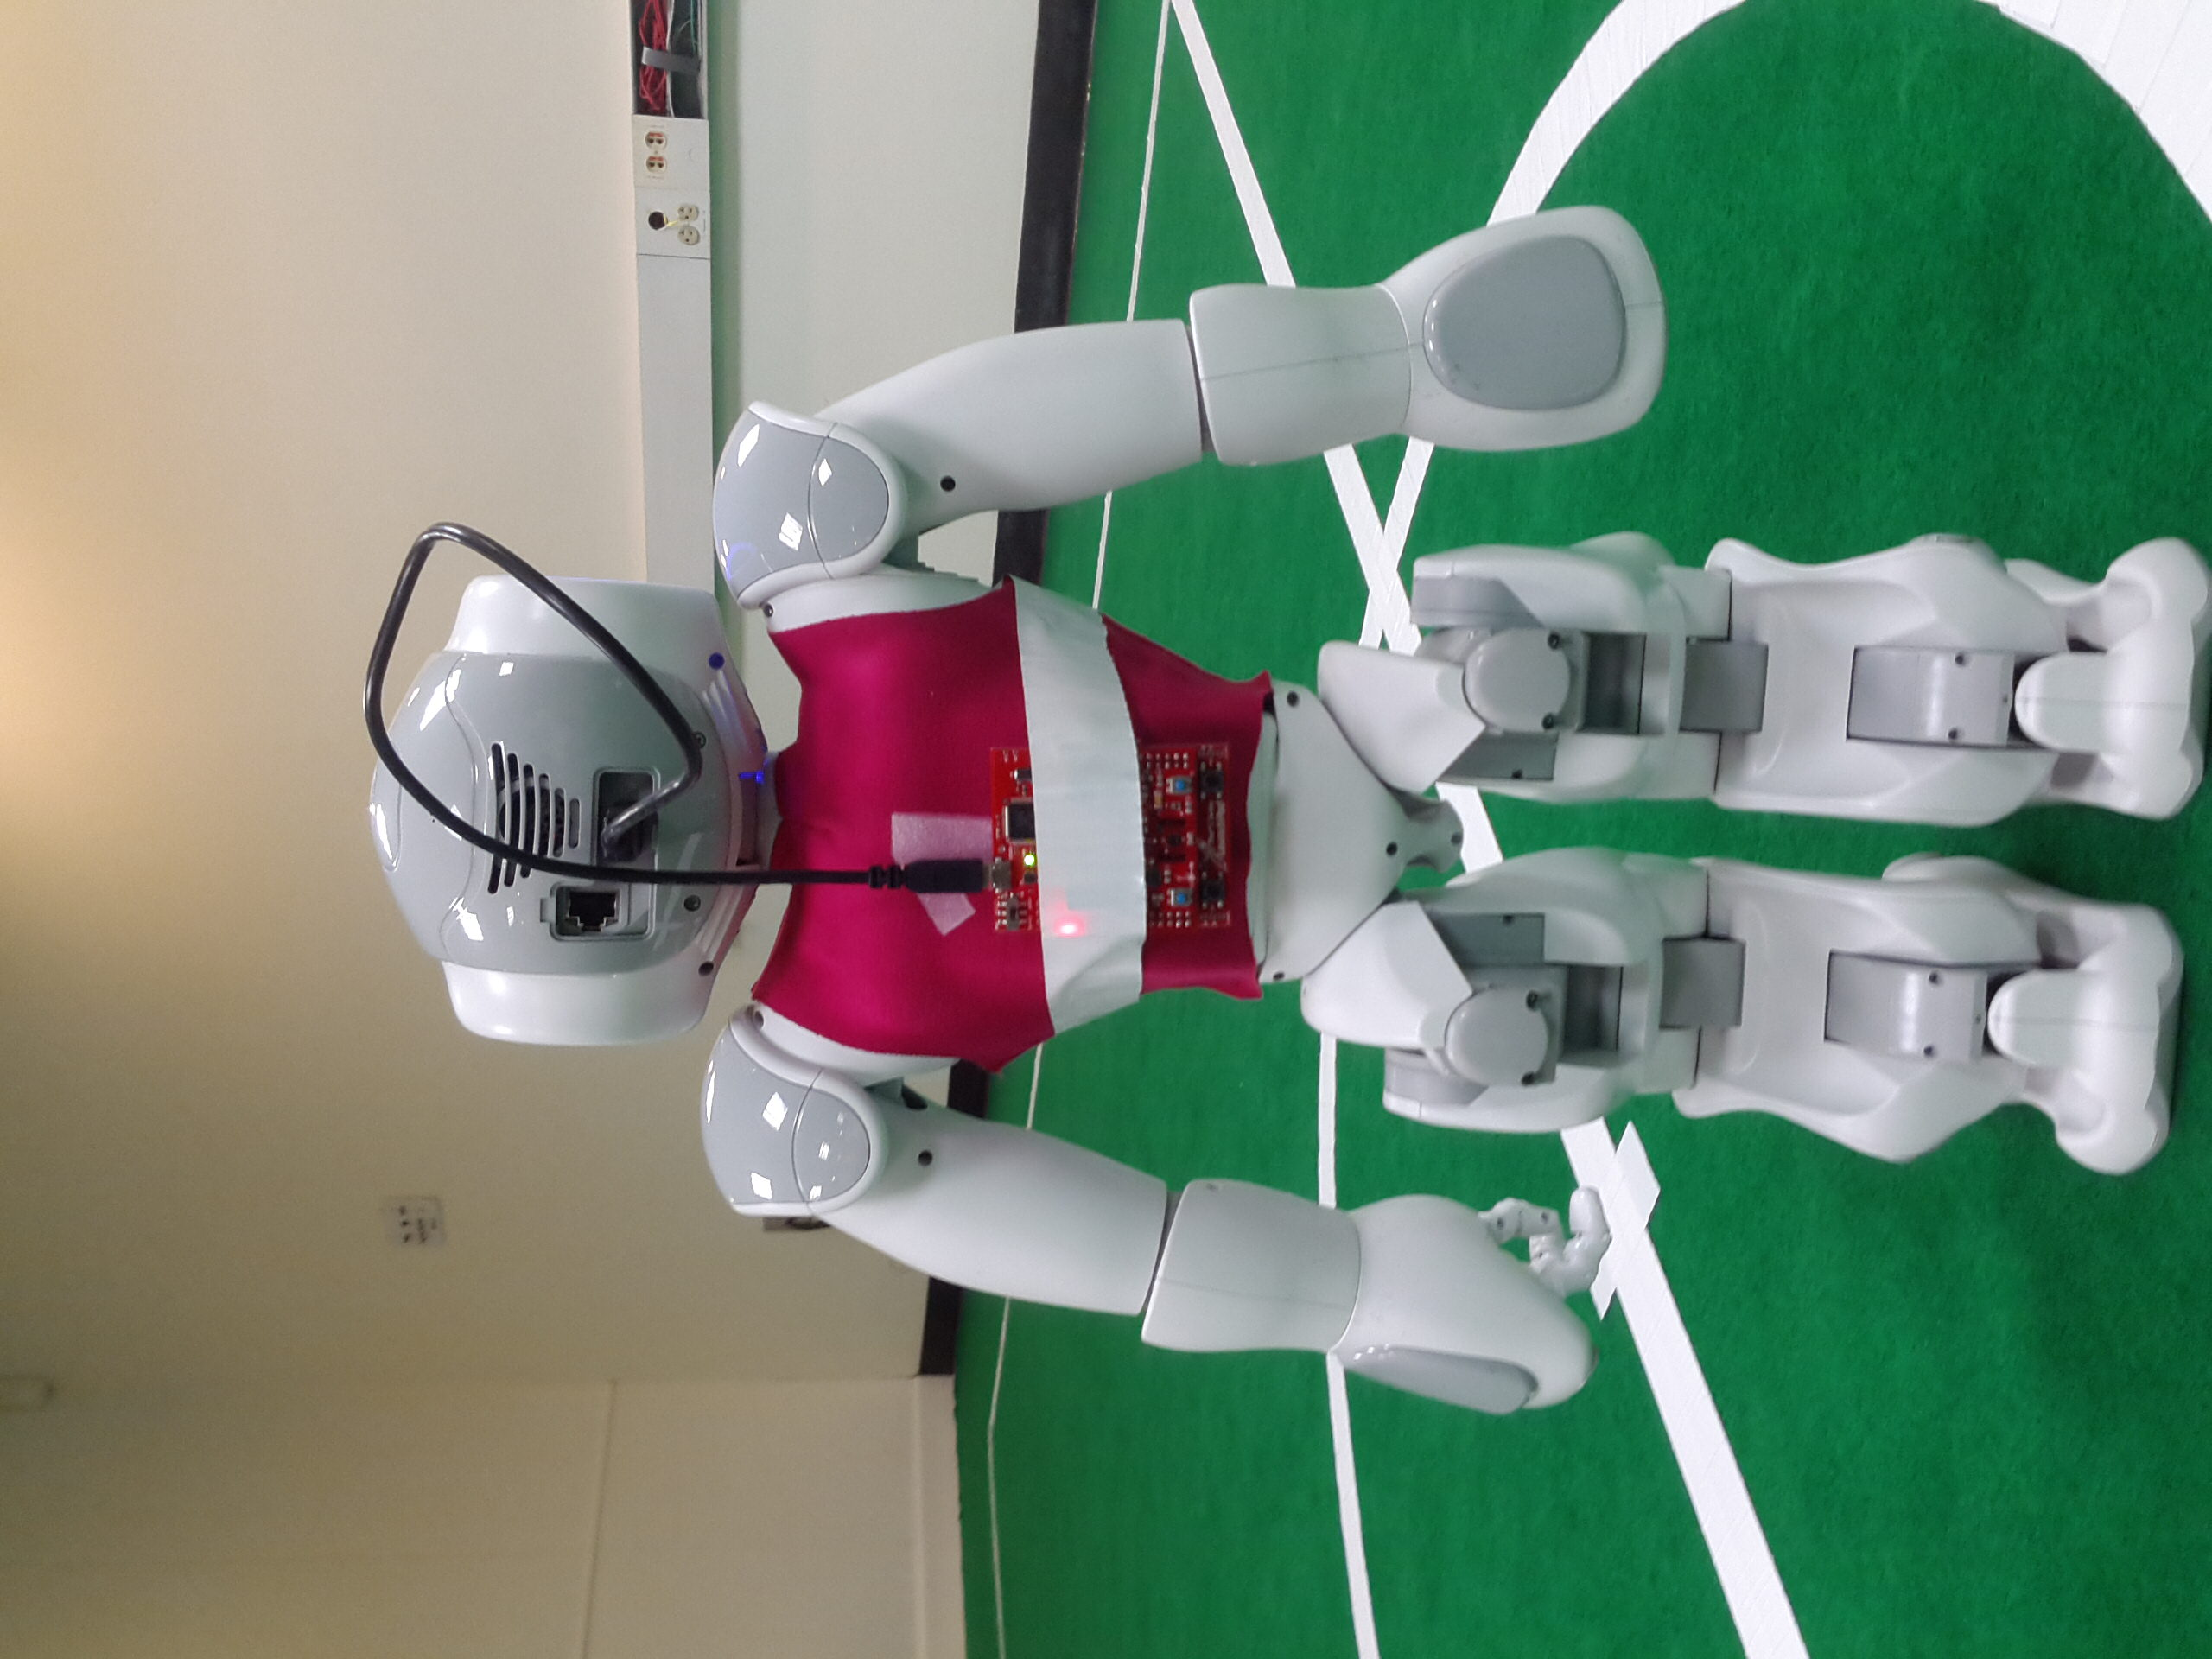
\includegraphics[width=0.5\textwidth] {attached_device}
 \caption{(a) Tiva C microcontroller with sensor bub was attached to the back of a NAO humanoid
robot; and (b) Sensor Hub BoosterPack. The roll is around x-axis, the pitch is around y-axis, and
the yaw is around z-axis.}
 \label{fig:attached_device}
\end{figure}
\vspace{-5mm}
We have configured InvenSense MPU-9150: 9-axis MEMS motion sensor on the sensor hub to sample data
at 50$Hz$. We have chosen this value to compensate delays in communications and to cope with the
constraints provided by the robot. We have used a threshold based method to detect the motions of
the robot. Specially, we have detected only the normal behaviors such as standing, walking, turning,
and falling behaviors such as falling back and front. Therefore, we have treated standing, walking
and turning as one event, while the falling as another event, which amounts to three events. Once
the thresholds were found from the data, we have increased the sampling rate of the device to 500 Hz
to detect the events swiftly.  

\begin{figure}[!t]
  \centering
  \subfloat[Marching.]{\label{fig:tsnedataset_1}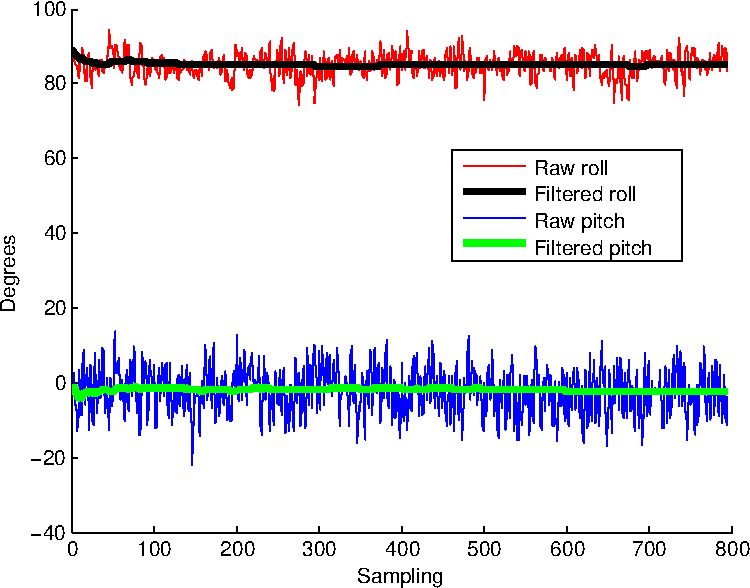
\includegraphics[width=0.45\textwidth]
       {plot1-crop}}
  \subfloat[Fast walk forward.]{\label{fig:tsnedataset_5}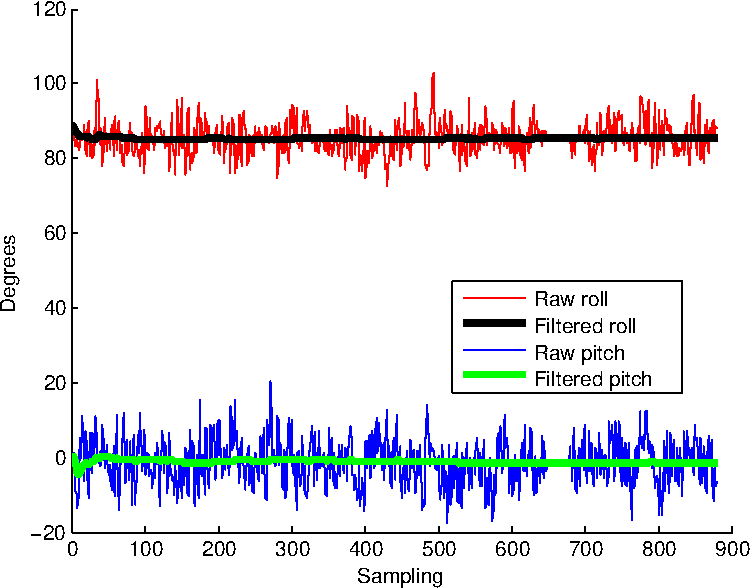
\includegraphics[width=0.45\textwidth]
       {plot2-crop}}
\\
  \subfloat[Slow walk backward.]{\label{fig:tsnedataset_7}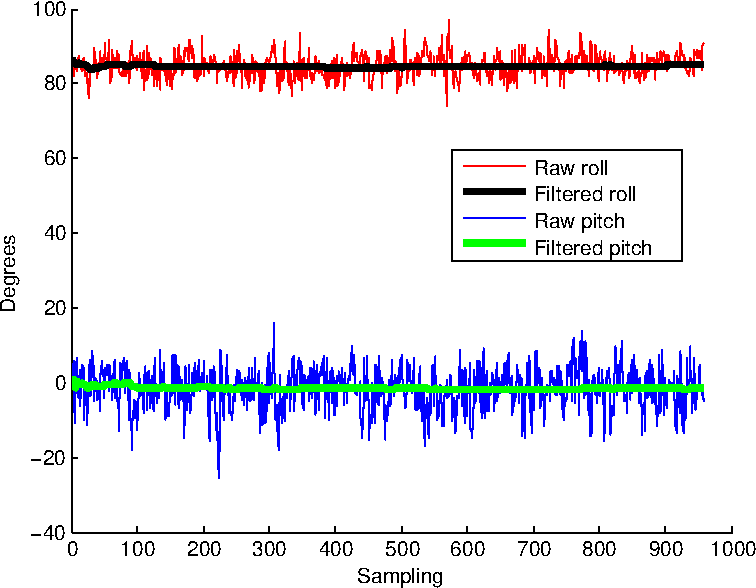
\includegraphics[width=0.45\textwidth]
       {plot3-crop}}
  \subfloat[Rotate
counter-clockwise.]{\label{fig:tsnedataset_8}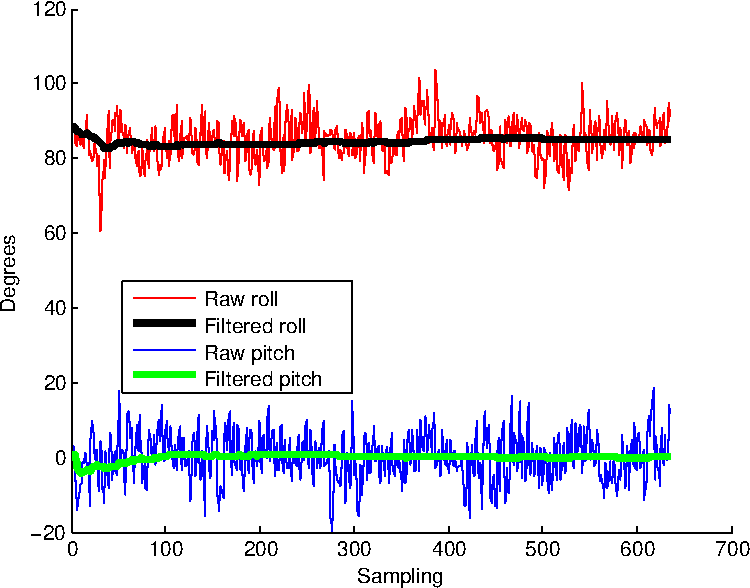
\includegraphics[width=0.45\textwidth]
       {plot4-crop}}
       \\
  \subfloat[Fast walk backward.]{\label{fig:tsnedataset_7}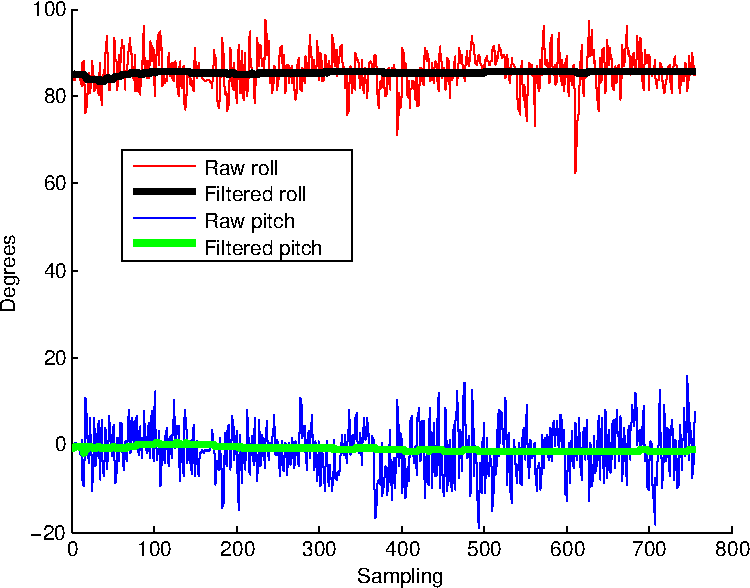
\includegraphics[width=0.45\textwidth]
       {plot5-crop}}
  \subfloat[Left side-way walk.]{\label{fig:tsnedataset_8}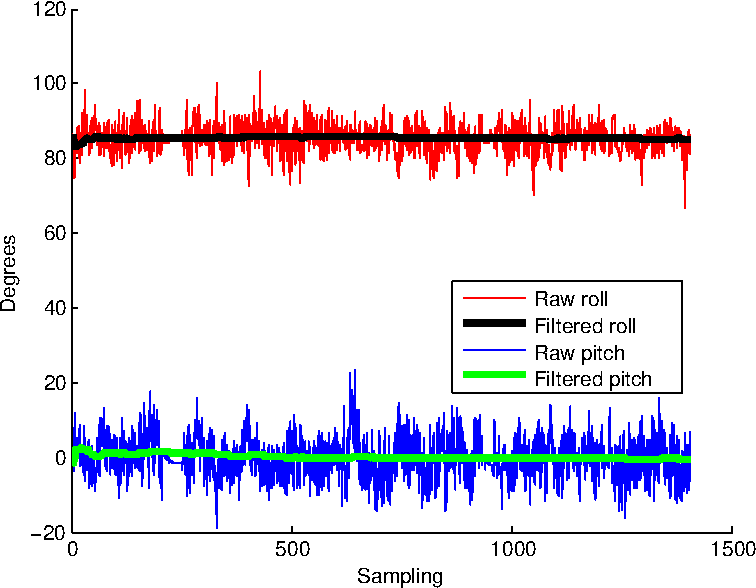
\includegraphics[width=0.45\textwidth]
       {plot6-crop}}
  \caption{The raw and filtered roll and pitch values for normal behaviors of NAO humanoid robot.}
  \label{fig:normalBehavior}
\vspace{-6mm}
\end{figure}

Our NAO robots run {\sf Robocanes} binary, which has been primarily written for soccer
playing. The walking engine of {\sf Robocanes} conducts primary movements. These movements are
regulated by linear speeds, $x_v$ and $y_v$, and a rotational speed $\theta_v$. Depending on these
values, we can let the robot walk (forward, backward, and side-ways), and rotate (clockwise and
counter-clockwise) with different speeds. Therefore, we have considered \begin{inparaenum}[(1)]
\item marching ($x_v = 0 , y_v = 0, \theta_v = 0$); \item fast walk forward/backward ($x_v = \pm200
, y v = 0, \theta_v = 0$); \item \item slow walk forward/backward ($x_v = \pm30 , y_v = 0, \theta_v
= 0$); \item side-way movements ($x_v = 0, y_v = \pm200, \theta_v = 0$); and  \item rotate
($x_v = 0 , y_v = 0, \theta_v = \pm 0.5$) \end{inparaenum} as normal behaviors. All other motions
are considered falling behaviors. 


We have used only the roll and the pitch values  to detect relevant events. In order to achieve an
effective threshold based decision making, first we have filtered the roll, pitch, and
yaw\footnote{Even though we have not used yaw values, we have filtered them using Kalman filter.}
values using a Kalman filter \cite{Welch:1995:IKF:897831}. Figure \ref{fig:normalBehavior} shows
the row and the filtered values of the row and the pitch values for marching, fast walk forward,
slow walk backward, rotate counter-clockwise, fast walk backward, and left side-way walk. Other
scenarios show similar plots, and we have refrained from plotting them. The threshold method
suggests that, if the filtered roll values are within the range $[90\pm15]$ (degrees) and the
filtered pitch values are within the rage $[0\pm15]$ (degrees), then 100\% accuracy the NAO humanoid
robot will show the normal behaviors. Otherwise, we can safely assume that the robot is in a fallen
state.   

There are four fallen states for the robot: \begin{inparaenum}[(1)] \item fallen
forwad; \item fallen backward; \item fallen to left side; and \item fallen to right
side\end{inparaenum}. Figure \ref{fig:fallenBehavior} shows the roll and pitch angles (row and
filtered) for typical fallen robot. If the filtered roll value is less that 60 degrees, we can
safely assume that the robot is fallen forward. If the filtered roll values is more than 100
degrees we can assume that the robot is fallen backward. To detect the events fallen to the left
and right, we have used the filtered pitch values. If the filtered pitch value is less than -50
degrees, we can assume that the robot is fallen to the left side, while if the filtered pitch
values is more than 50 degrees, we can assume that the robot is fallen to the right side. With
these thresholds for a separate test cases, the thresholding method has detected fallen state 100\%
accuracy. 

\begin{figure}[!t]
  \centering
  \subfloat[Fallen forward.]{\label{fig:tsnedataset_1}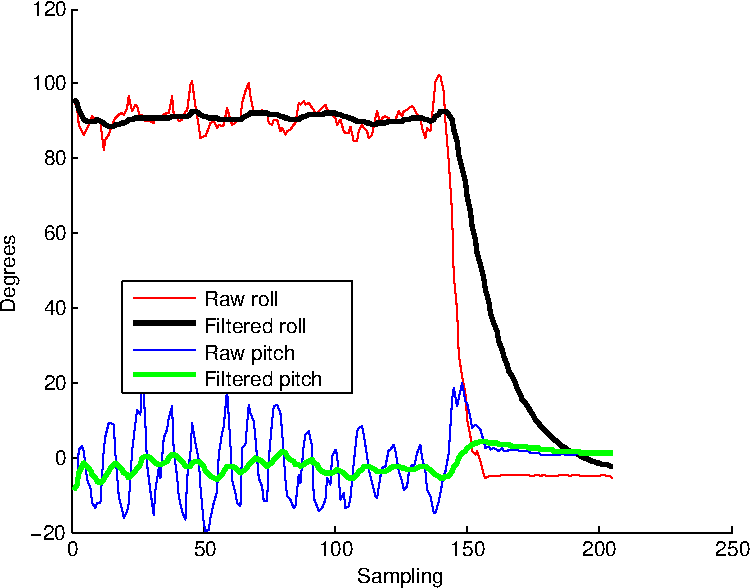
\includegraphics[width=0.45\textwidth]
       {plot1_fallen-crop}}
  \subfloat[Fallen backward.]{\label{fig:tsnedataset_5}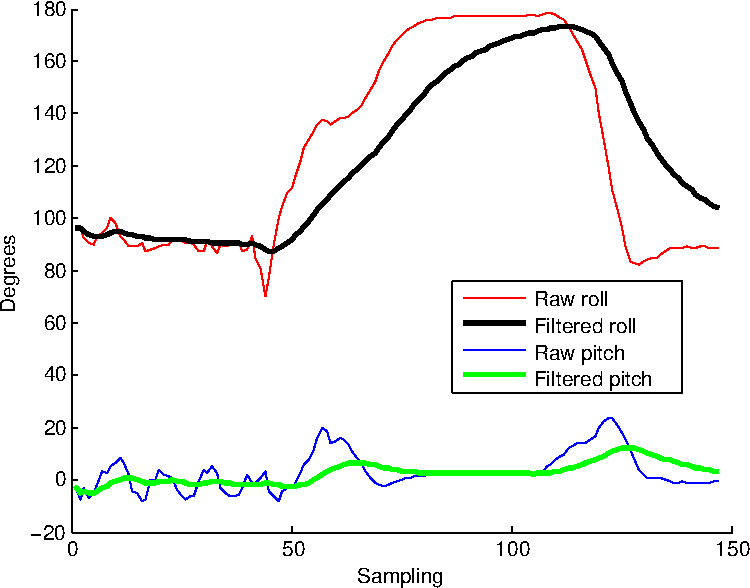
\includegraphics[width=0.45\textwidth]
       {plot2_fallen-crop}}
\\
  \subfloat[Fallen to left side.]{\label{fig:tsnedataset_7}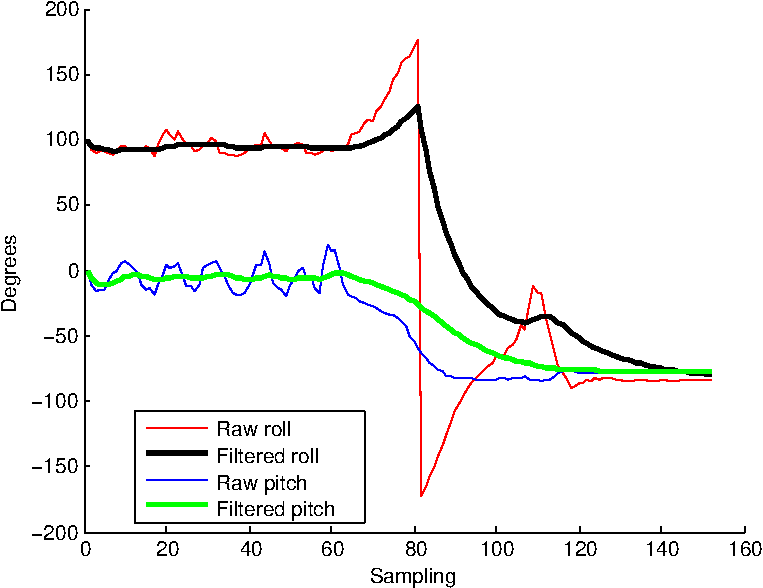
\includegraphics[width=0.45\textwidth]
       {plot3_fallen-crop}}
  \subfloat[Fallen to right
side.]{\label{fig:tsnedataset_8}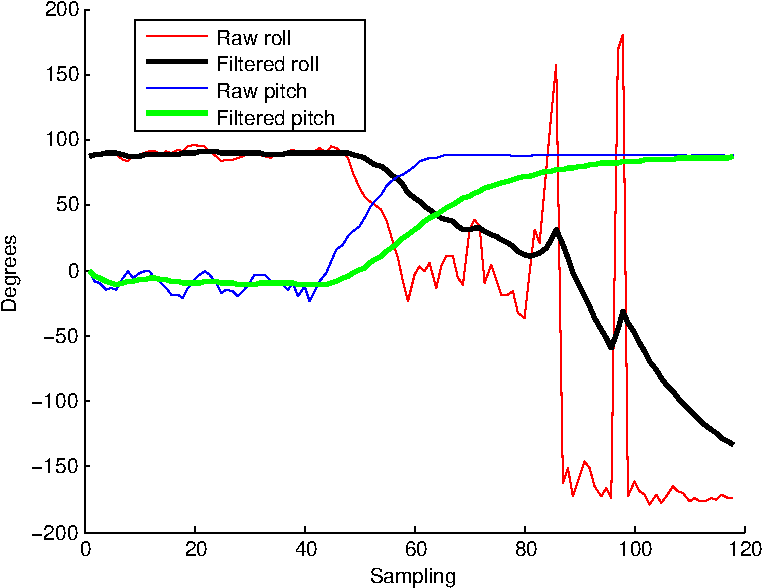
\includegraphics[width=0.45\textwidth]
       {plot4_fallen-crop}}      
  \caption{The raw and filtered roll and pitch values for fallen states of NAO humanoid robot.}
  \label{fig:fallenBehavior}
\vspace{-6mm}
\end{figure}

The range of motion of NAO robot is comparatively limited compared to a able-bodied human.
Therefore, we are able to obtain satisfactory results for detecting motion event from the
thresholding method. In future, we are planning to detect specific events such as walking forward
(fast/slow), and rotating separately. When determining the results, we have sampled the motion
device data at the rate 50$Hz$. During operation, using the same thresholds, we can sample the
motion device at higher rates. In future, we are also planning to learn online from accelerometer,
gyroscope, and magnetometer instead of Euler angles. Even though Euler angles have singularities,
for our experiments, we operate the device avoiding those singularities.  


\section{Related Work}

The microcontrollers and embedded devices provide a flexible platform to build may real world
applications. In order to build these applications, a practitioner would require  flexible and
reliable software solutions. A practitioner also may require to use more than one functionality
provided by the devices to build applications. Energia and TIs software solutions provide
facilities to build applications to a certain degree, but, they lack methods or systems to integrate
multiple devices simultaneously without much user burden. In the project, we have provided a
state-of-the-art open source software solution to build heterogeneous applications on many devices,
programmed on multiple operating systems. To our knowledge, our open source software solution is the
first of its kind. 

There has been an increasing interest in detecting human motions using embedded devices. Woon-Sung
et. al. \cite{baek2013real} proposed  a fall  detection  system  using necklace-shaped tri-axial
accelerometer  and  gyroscope  sensors  to  classify  the  behavior  and  posture  of  the detection
 subject. They claim that their  approach  can  successfully  distinguish between  ADL and  fall, 
with  sensitivities  greater  than  80 \%  and specificities  of  100\%. Ying-Wen et. al.
\cite{bai2013recognition} proposed an activity monitoring system based on smart phone sensor
reading and they claim that they can identify human activity with high degree of accuracy. Leno et.
al. \cite{leone2013supervised} prosed a system to detect event that cause trauma, and disabilities
using a tri-axial MEMS wearable wireless accelerometer. They have used support vector machine for
robust classification of different events. There has been similar efforts to detect human motions
using motion tracking, e.g., \cite{dumitrache2013fall,kumarwearable,liang2012pre}.

Compared the existing methods, we have investigated the possibility of using our software solution
to detect human motions and human-like motions from able-bodied humans and NAO humanoid robot. To
our knowledge, we are the first to investigate the prospect of using an external embedded device to
detect human-like motions on a NAO humanoid robot. 

\section{Conclusion}

In this project, we have proposed an open source software solution to write heterogeneous
applications on TIs microcontrollers. We have used our software solution to detect motions on
able-bodied humans and NAO humanoid robots. We have shown that our methods are capable of detecting
motions with high accuracy. We have used machine learning methods and thresholding methods to
detect different motions and provided justifications for the success of the applications. 

\bibliographystyle{splncs03}
\bibliography{references}

\newpage
\section*{Appendix: Implementation}
\label{appendix:Implementation}
CSC688 Energia framework primarily consists of three files: \begin{inparaenum}[(1)] \item
\label{fmw:A} {\sf Template.h}; \item \label{fmw:B} {\sf Framework.h}; and \item \label{fmw:C} {\sf
Framework.cpp}\end{inparaenum}. A practitioner can only need to use these three files to get the
complete functionality of the framework. The framework has been tested on Taxas Instruments MSP430,
Stellaris, and the Tiva C LaunchPad boards. In order to compile the project:

\begin{itemize}
 \item Online (microcontrollers):
\begin{enumerate}
\item connect the microcontroller,
\item download the latest Energia distribution that matches to the host machine,
\item open {\sf csc688.ino} file, and 
\item compile and upload the {\sf csc688.elf} file to the microcontroller.
\end{enumerate}

\item Offline:
\begin{enumerate}
\item start {\sf ./configure\_offline} script to generate make file,
\item execute command {\sf make},
\item change the directory to {\sf build}, and 
\item execute the binary {./offline\_csc688}.
\end{enumerate}

\item Visualizations:
\begin{enumerate}
\item our visualization uses QT4 library. Therefore, download the latest QT4 library to your host
system,
\item change the directory to {\sf viz},
\item execute command {\sf qmake viz.pro},
\item execute command {\sf make},
\item change the directory to {\sf build}, and 
\item execute the binary {\sf viz}.
\end{enumerate}

\end{itemize}


To write modules and representations, the practitioner needs to include the three C\texttt{++}
files \ref{fmw:A}, \ref{fmw:B}, and \ref{fmw:C}. The following example shows the implementation
of the module {\sf TestModule1} and the representation {\sf TestRepresentation1} in Figure
\ref{fig:framework}.

\begin{figure}[!ht]
\begin{center}
\begin{minted}[mathescape, linenos=false, fontsize=\small]{c++}
// -----------------------------------------------------------------
#pragma once

#include "Template.h"

REPRESENTATION(TestRepresentation1)
class TestRepresentation1: public TestRepresentation1Base
{
public:
  bool rightButton, leftButton;
  TestRepresentation1() :
    rightButton(false), leftButton(false)
  {
  }
};
// ------------------------------------------------------------------
\end{minted}
\end{center}
\captionof{listing}{{\sf TestRepresentation1.h}}
\label{list:TestRepresentation1.h}
\end{figure}

Listing \ref{list:TestRepresentation1.h} shows the implementation of the representation {\sf
TestRepresentation1}. This representation shares the button state information of Tiva C among
modules. {\sf Template.h} C\texttt{++} header file provides the macro {\sf REPRESENTATION} to
register the representation with the framework, only if, a module provides the given
representation. 

\begin{figure}[!ht]
\begin{center}
\begin{minted}[mathescape, linenos=false, fontsize=\small]{c++}
// -----------------------------------------------------------------
#pragma once

#include "Template.h"
#include "LaunchPadRepresentation.h"
#include "TestRepresentation1.h"

MODULE(TestModule1)
  REQUIRES(LaunchPadRepresentation)
  PROVIDES(TestRepresentation1)
END_MODULE

class TestModule1: public TestModule1Base
{
  public:
    void update(TestRepresentation1& theTestRepresentation1);
}; 
// -----------------------------------------------------------------
\end{minted}
\end{center}
\captionof{listing}{{\sf TestModule1.h}}
\label{list:TestModule1.h}
\end{figure}

Listing \ref{list:TestModule1.h} shows the header file {\sf TestModule1.h}. This class schedules
the functionalities of a module. {\sf Template.h} defines the macros {\sf MODULE}, {\sf REQUIRES},
{\sf PROVIDES}, {\sf USES}, {\sf END\_MODULE}, and {\sf MAKE\_MODULE}.  {\sf REQUIRES} requests a
representation from another module, while {\sf PROVIDES} provides a representation from a given
module. {\sf USES} requests a representation from anywhere in the graph, without infringing the
topology of the topologically sorted graph. {\sf MODULE} and {\sf END\_MODULE} generates a base
class (e.g.,{\sf TestModule1Base}) for the module (e.g., {\sf TestModule1}) that will be used by the
framework. Since, this module provides the representation {\sf TestRepresentation1}, it needs to
implement the method \mintinline{c++}{public: void update(TestRepresentation1&
theTestRepresentation1)}. This module also requires the representation {\sf
LaunchPadRepresentation}. According to Figure \ref{fig:framework}, it is provided by the module
{\sf LaunchPadModule}. 


\begin{figure}[!ht]
\begin{center}
\begin{minted}[mathescape, linenos=false, fontsize=\small]{c++}
// -----------------------------------------------------------------
#include "TestModule1.h"

void TestModule1::update(TestRepresentation1& theTestRepresentation1)
{
  theTestRepresentation1.leftButton = 
                          theTestRepresentation1.rightButton = false;
#if defined(ENERGIA)
  if (digitalRead(PUSH1) == LOW)
    theTestRepresentation1.leftButton = true;
  if (digitalRead(PUSH2) == LOW)
    theTestRepresentation1.rightButton = true;
#endif
}

MAKE_MODULE(TestModule1)
// -----------------------------------------------------------------
\end{minted}
\end{center}
\captionof{listing}{{\sf TestModule1.cpp}}
\label{list:TestModule1.cpp}
\end{figure}


Listing \ref{list:TestModule1.cpp} shows the implementation of the module {\sf TestModule1}.  The
macro {\sf MAKE\_MODULE} registers the module {\sf TestModule1} with the framework. According to
Figure \ref{fig:framework}, the module {\sf TestModule2} requests representations provided by {\sf
TestModule1}. Please refer to the documentation of CSC688 Energia for more examples and usages
(\url{https://github.com/samindaa/csc688}).  




\end{sloppy}
\end{document}